USARSim is designed to communicate over an American Standard Code for Information Interchange (ASCII) Transmission Control Protocol/Internet Protocol (TCP/IP) socket with a host computer. The host computer initiates the socket interface and creates the desired robot in the simulated world that is currently running on the game server. A robot's configuration is controlled by an initialization file that resides on the simulation system's computer. This file controls such aspects as sensor configuration, battery life, and simulated noise models. Please see the USARSim wiki for more information on robot configuration~\cite{USARSimWeb}.  One socket connection is established per simulated robot, with both commands and sensor data being transmitted over the socket. An additional separate socket is established for high-volume sensors such as camera systems.

ROS stacks are designed with their lowest-level node at a hardware abstraction layer that provides basic topics to and from the robot. For example, the mobility stack expects to control a platform by writing commands to low-level topics that control items such as platform velocities, and to receive feedback from sensors over other low-level topics. These stacks may also place constraints or naming conventions on the topics.  In order to close this low-level loop between ROS and USARSim, a USARSim package was created. This package contains a node called {\it RosSim} that publishes a ROS transform tree (from the ROS {\it tf} package) and sensor messages, and also accepts platform and actuator motion commands. When run, it provides a mechanism for spawning a robot in USARSim, and then auto-discovering the robot's sensors, actuators, and drive configuration in order to provide the necessary ROS topics. 
 \begin{table}[t!]
    \begin{center}
    \small{
    \begin{tabular}{ | l | l | p{4cm} |}
    \hline
    Parameter & Default & Definition \\ \hline
   robotType & P3AT & Type of robot to spawn. \\ \hline
   hostname & localhost & Name of host running USARSim. \\ \hline
   port & 3000 & TCP/IP Port on which USARSim listens. \\ \hline
   startPosition & Vehicle1 & Named location where robot should be spawned. This location is simulated world dependent. \\ \hline
   odomSensor & InsTest & Odometry sensor that should be used as the default sensor for feeding the {\it odom} topic of ROS.\\ \hline
    \end{tabular}
   }
    \caption{Parameters for USARSim ROS node.}
    \label{Table:USARSimNode}
    \end{center}
\end{table}
\begin{figure}[t!]
\centering
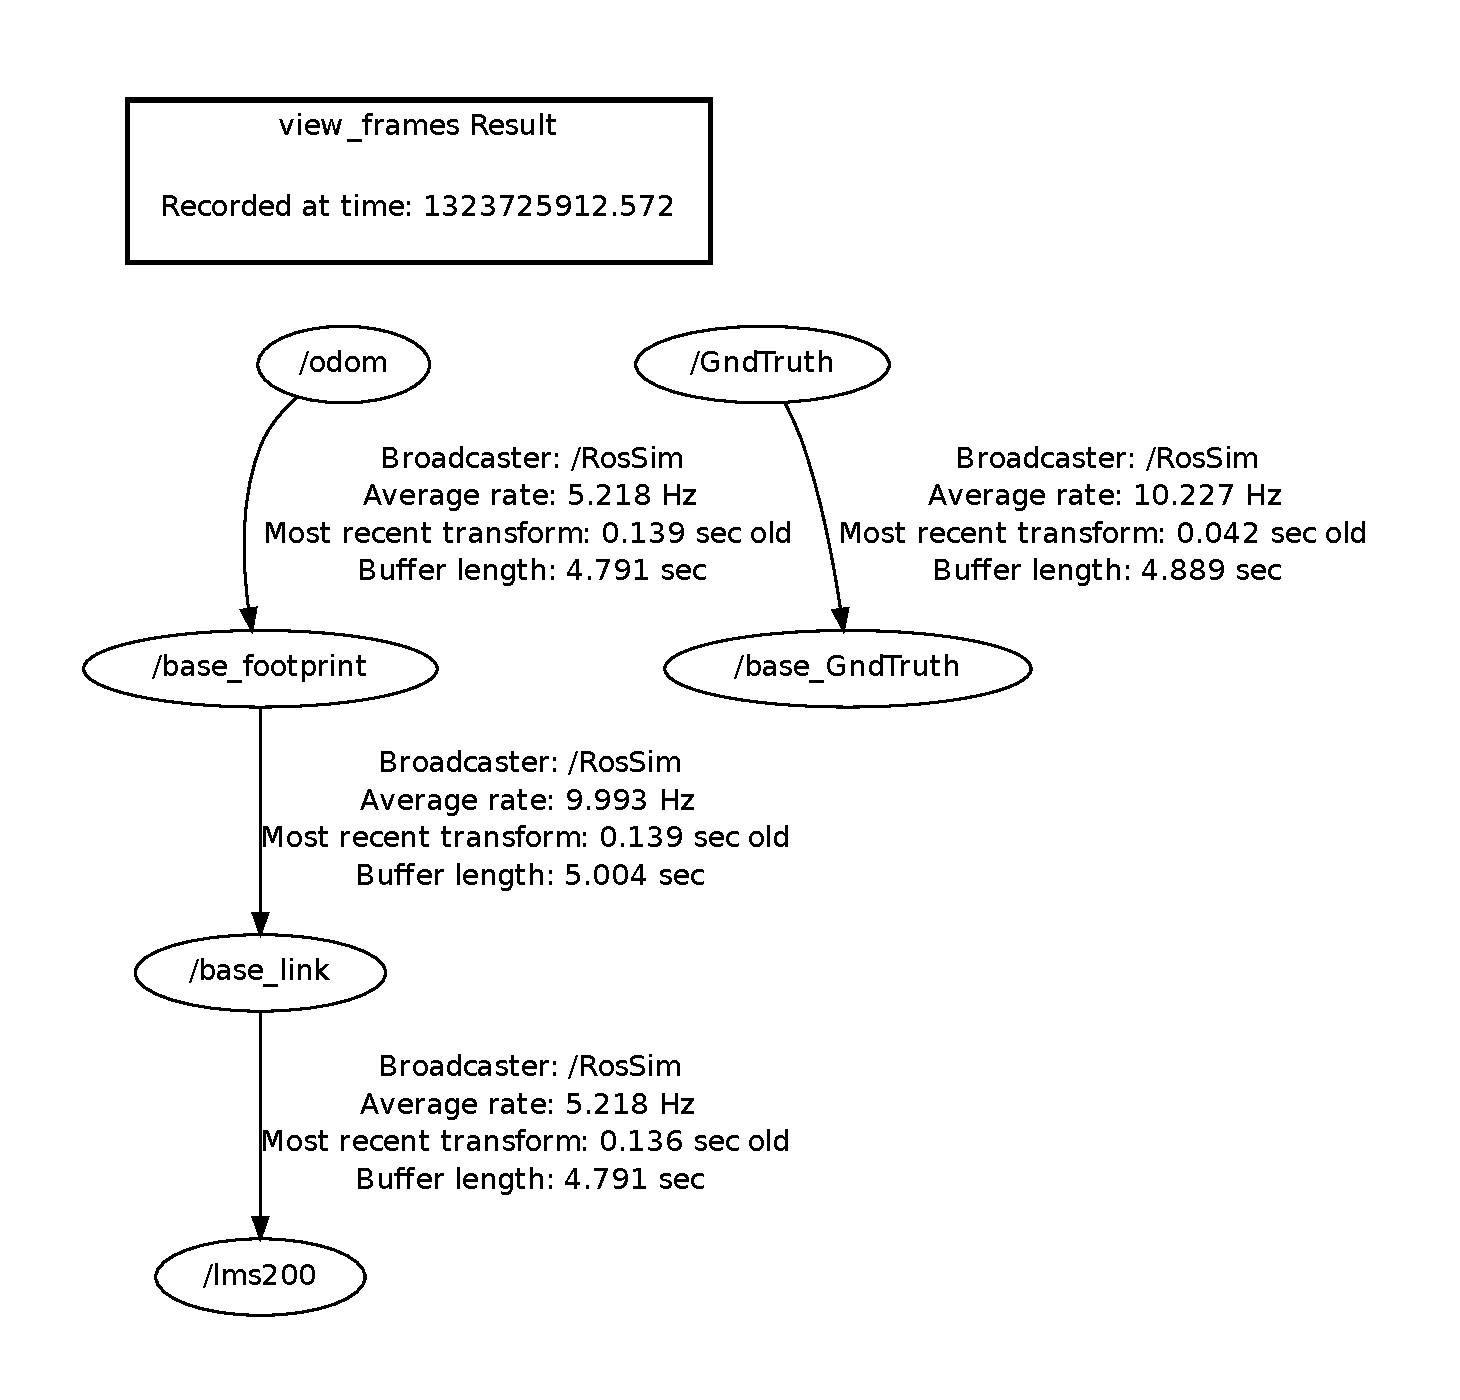
\includegraphics[width=8cm]{Figures/ROS/P3ATFrames.pdf}
\caption{Auto-generated tf Transform tree for P3AT robot.}
\label{Fig:P3ATTransformTree}
\end{figure}

The {\it RosSim} node relies on several parameters for its configuration. These are detailed in Table~\ref{Table:USARSimNode}, and provide information necessary for the creation of a robot in USARSim and a transform tree in ROS. A transform tree for the P3AT robot is shown in Figure~\ref{Fig:P3ATTransformTree}. This transform tree is built automatically from data obtained from the USARSim geometry {\it geo} and configuration {\it conf} messages. Since USARSim supports more than one localization sensor on a robot, the {\it odomSensor} parameter is consulted to determine which sensor should be built into the tree. That sensor's name is automatically changed to {\it odom}. The {\it base\_footprint}, representing the robot platform and the {\it base\_link}, representing robot sensor mounting points, are also automatically generated. Additional localization sensors (e.g., the ground truth sensor for the P3AT robot) are provided with their own transform tree.

Vehicle movement commands into USARSim vary depending on the robot type. For example, skid-steered vehicles require left and right wheel velocities while Ackerman steered vehicles required steering angle and linear velocity. ROS provides a {\it cmd\_vel} topic that includes both linear and angular velocities. The {\it RosSim} node automatically converts these velocities into the appropriate commands and values for the USARSim simulator based on the robots steering type, wheelbase, and wheel separation. Vehicle speeds are also clamped to not exceed maximum velocities that are set in the simulation.
